\chapter{Plotting}

\mlab is very powerful for producing both \twod and \threed plots. Plots can be created and manipulated interactively or by commands. \mlab offers a number of different formats for exporting plots, including EPS (Encapsulated PostScript), PDF (Portable Document Format) and JPEG (Joint Photographic Experts Group), so you can easily include \mlab plots in your reports.

\section{Simple \twod plotting}
The simplest and most commonly used plotting command is \mcode{plot(x,y)}, where \mcode{x} and \mcode{y} are simply vectors containing the $x$ and $y$ coordinates of the data to be plotted. Listing~\ref{lst:simple_plot} demonstrates the commands used to create a plot of the function, $f(x) = e^{-\frac{x}{10}} \sin(x)$, which is shown in Figure~\ref{fig:simple_plot}.
\begin{lstlisting}[caption={A simple plot},label=lst:simple_plot]
>> x = 0:0.1:20;
>> y = exp(-x/10).*sin(x);
>> plot(x,y), grid on, xlabel('x'), ...
ylabel('f(x) = e^{-x/10} sin(x)'), title('A simple plot')
\end{lstlisting}
\begin{figure}
	\myfloatalign
	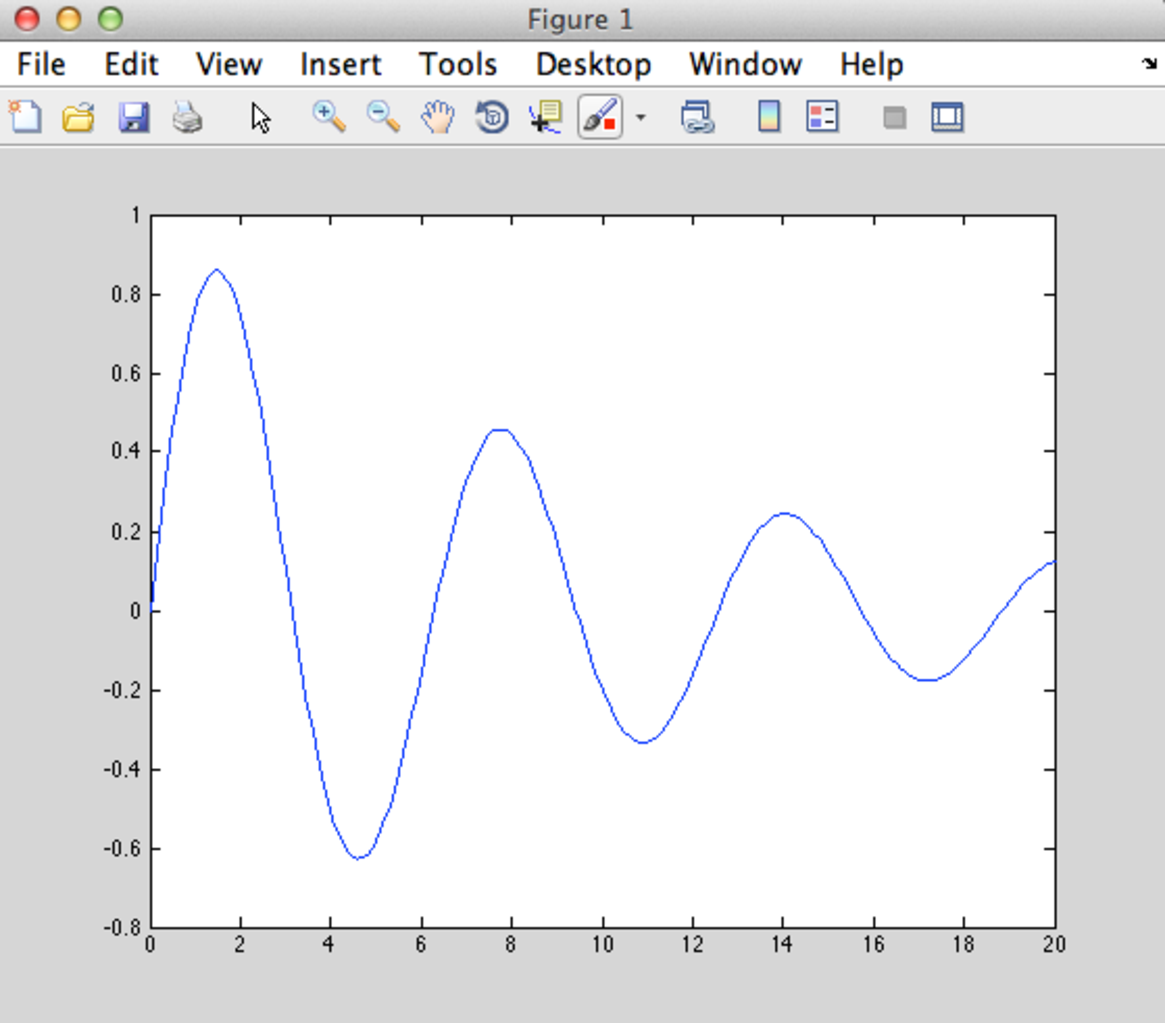
\includegraphics[width=0.9\linewidth]{Graphics/Unit02/simple_plot}
	\caption{Plot of $f(x) = e^{-\frac{x}{10}} \sin(x)$}
	\label{fig:simple_plot}
\end{figure}

\subsubsection{Comments:}
\begin{itemize}
\item The vectors containing the \mcode{x} and \mcode{y} data must be the same length.
\item The plot command can be used to plot multiple sets of data on the same axes, \ie\ \mcode{plot(x1,y1,x2,y2)}.
\item The dot-dot-dot \mcode{...} (ellipsis) notation is used to indicate that Lines 3 and 4 are one long line. The ellipsis notation just allows the line to be broken to make it more readable. Each comma-separated command could also have been typed on a separate line. 
\end{itemize}
When \mlab executes a plotting command, a new Figure Window opens with the plot in it. The following list gives the most common commands for changing plot properties.
\begin{itemize}
\item \mcode{grid on} displays the grid!
\item \mcode{xlabel('My x-axis label')}, \mcode{ylabel('My y-axis label')}, and \mcode{title('My title')} can be used to label the corresponding parts of the plot. You must enclose your labels with single quotes which denotes a string of text.
\item \mcode{legend('Data1','Data2')} is used to place a legend and label the data-sets when you have multiple data-sets on one plot.
\item You can specify line style and colour within the \mcode{plot} command \eg\ \mcode{plot(x1,y1,'b-',x2,y2,'r--')}. This command would make the first data-set a solid blue line, and the second data-set a dashed red line. Tables~\ref{tab:plot_line_styles}--\ref{tab:plot_colours} gives some of the most common line styles and colours.
\end{itemize}

\begin{table}[h]
	\caption{Line styles in plots}
	\label{tab:plot_line_styles}
	\myfloatalign
	\begin{tabular}{ll}\toprule
	\spacedlowsmallcaps{String specifier} & \spacedlowsmallcaps{Line style}\\ \midrule
	\mcode{-} & Solid line (default) \\
	\mcode{--} & Dashed line \\
	\mcode{:} & Dotted line \\
	\mcode{-.} & Dash-dot line \\
	\bottomrule
	\end{tabular}
\end{table}

\begin{table}[h]
	\caption{Colours in plots}
	\label{tab:plot_colours}
	\myfloatalign
	\begin{tabular}{ll}\toprule
	\spacedlowsmallcaps{String specifier} & \spacedlowsmallcaps{Line colour}\\ \midrule
	\mcode{r} & Red \\
	\mcode{g} & Green \\
	\mcode{b} & Blue (default) \\
	\mcode{w} & White \\
	\mcode{k} & Black \\
	\bottomrule
	\end{tabular}
\end{table}

Plot properties can also be manipulated interactively (without having to issue commands) by clicking on the \textit{Show Plot Tools} icon in the Figure Window toolbar, shown in Figure~\ref{fig:interact_icon}. Properties such as the axis limits, gridlines, line style, colour and thickness, text font type and size, and legend \etc\ can all be adjusted be clicking on the appropriate parts of the plot. \\
\begin{figure}[h]
	\myfloatalign
	
\includegraphics[width=0.9\linewidth]{Graphics/Unit02/interact_icon}
	\caption{\textit{Show Plot Tools} toolbar icon in Figure Window}
	\label{fig:interact_icon}
\end{figure}

\addtolength{\parindent}{-4mm}
\fcolorbox{myborderblue}{myblue}{%
\begin{minipage}{\linewidth}
\begin{minipage}{6mm}

\includegraphics[scale=0.03]{Graphics/General/help_icon}
\end{minipage}
\textit{Producing good plots} \\
Whether you manipulate your plots via commands or interactively, here is some useful advice for producing good plots in \mlab.
\begin{itemize}
\item Give your plot an informative title \\ \eg\ \mcode{title('Stress vs. strain of steel')}
\item Label your axes and remember to include units where appropriate \\ \eg\ \mcode{xlabel('Strain'), ylabel('Stress (MPa)')}
\item Use line colours and styles carefully so that multiple data-sets can be easily distinguished \eg\ \mcode{plot(x1,y1,'b-',x2,y2,'r--'), grid on}
\item Remember to insert a legend when you are plotting multiple data-sets on one plot \eg\ \mcode{legend('Carbon steel','Stainless steel')}
\end{itemize}
\end{minipage}%
}\\
\addtolength{\parindent}{4mm}
\vspace{5mm}

%%%%%%%%%%%%%%%%%%%%%%%%%%%%%%%%%%%%%%%%%%%%%%
% Screencast: Creating a simple plot
%%%%%%%%%%%%%%%%%%%%%%%%%%%%%%%%%%%%%%%%%%%%%%
\addtolength{\parindent}{-4mm}
\fcolorbox{myborderblue}{myblue}{%
\begin{minipage}{\linewidth}
\begin{minipage}{6mm}

\includegraphics[scale=0.03]{Graphics/General/screencast_icon}
\end{minipage}
\href{http://www.eng.ed.ac.uk/teaching/courses/matlab/unit02/simple-plot.shtml}{\screencast{Creating a simple plot}}\\
(http://www.eng.ed.ac.uk/teaching/courses/matlab/unit02/simple-plot.shtml)
\end{minipage}%
}\\
\addtolength{\parindent}{4mm}

\mlab has many built-in plot types, and a great way of getting a quick overview of all the different plot types is to select a variable in your Workspace Browser, click on the disclosure triangle next to the \textit{plot} toolbar icon and select \textit{More plots...}, as shown in Figure~\ref{fig:access_plot_catalog}. This will launch the \textit{Plot Catalog} shown in Figure~\ref{fig:plot_catalog}.
\begin{figure}[h]
	\myfloatalign
	\subfloat[Accessing the \textit{Plot Catalog}]
	%%%% Changed width from 0.45 AG 23/01/2014 %%%%
    {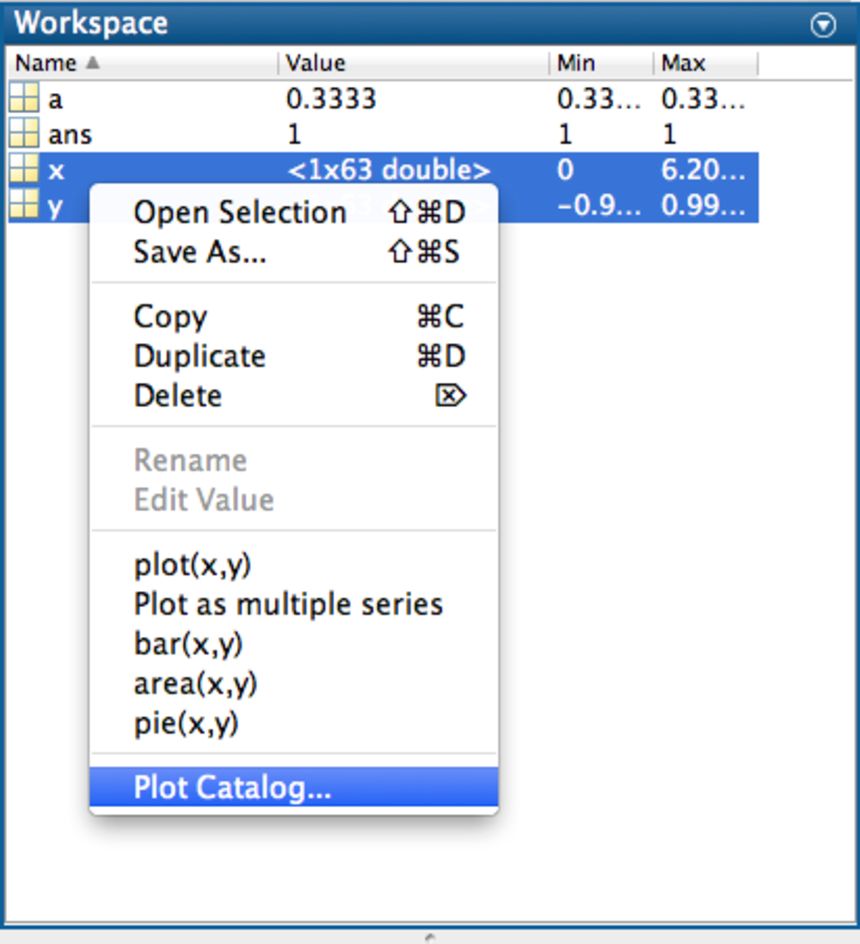
\includegraphics[width=0.45\linewidth]{Graphics/Unit02/access_plot_catalog}\label{fig:access_plot_catalog}} \\
    \subfloat[The \textit{Plot Catalog}]
    {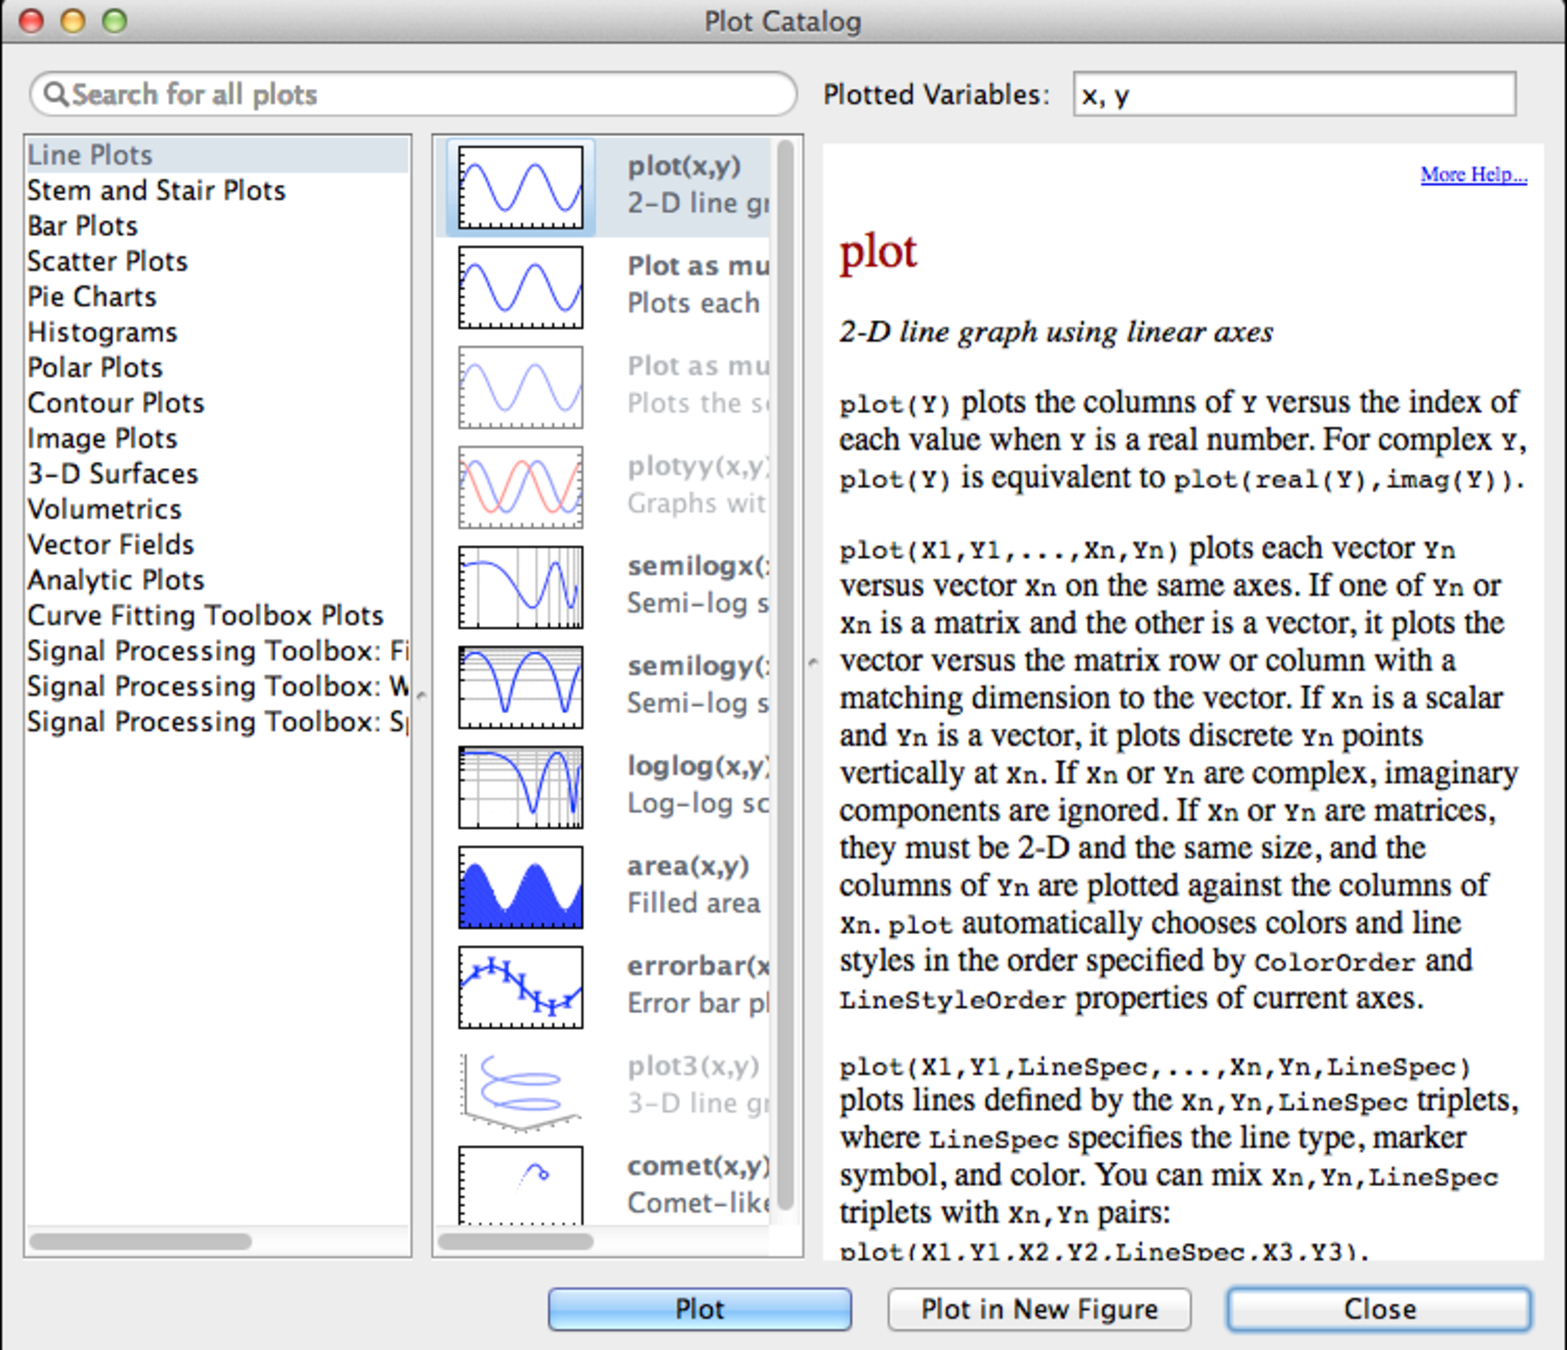
\includegraphics[width=\linewidth]{Graphics/Unit02/plot_catalog}\label{fig:plot_catalog}}
    \caption{\textit{The Plot Catalog}}
\end{figure}

%%%%%%%%%%%%%%%%%%%%%%%%%%%%%%%%%%%%%%%%%%%%%%
% Screencast: Plotting experimental data
%%%%%%%%%%%%%%%%%%%%%%%%%%%%%%%%%%%%%%%%%%%%%%
\addtolength{\parindent}{-4mm}
\fcolorbox{myborderblue}{myblue}{%
\begin{minipage}{\linewidth}
\begin{minipage}{6mm}

\includegraphics[scale=0.03]{Graphics/General/screencast_icon}
\end{minipage}
\href{http://www.eng.ed.ac.uk/teaching/courses/matlab/unit02/plot-exp-data.shtml}{\screencast{Plotting experimental data}}\\
(http://www.eng.ed.ac.uk/teaching/courses/matlab/unit02/plot-exp-data.shtml)
\end{minipage}%
}\\
\addtolength{\parindent}{4mm}
\vspace{5mm}

\addtolength{\parindent}{-4mm}
\fcolorbox{myborderblue}{myblue}{%
\begin{minipage}{\linewidth}
\begin{minipage}{6mm}

\includegraphics[scale=0.03]{Graphics/General/help_icon}
\end{minipage}
\textit{Importing data from external sources} \\
You can import data from other programs into \mlab using the \textit{Copy \textrightarrow Paste} method, or using the \textit{Import Data Wizard}, found at \textit{File \textrightarrow Import Data...}, for Microsoft Excel data, Comma-separated value files and more. There are also functions, \mcode{xlsread} and \mcode{xlswrite}.
\end{minipage}%
}\\
\addtolength{\parindent}{4mm}

\subsection{Multiple plots in one Figure Window}
The \mcode{subplot} command can be used to display a number of different plots in a single Figure Window, as shown in Figure~\ref{fig:subplots}. The \mcode{subplot} command takes three arguments that determine the number and location of plots in the Figure Window. For example, \mcode{subplot(2,2,1)} specifies that the Figure Window will be divided into 2 rows and 2 columns of plots, and selects the first subplot to plot into. Listing~\ref{lst:subplots} shows an example of usage of the \mcode{subplot} command.
\begin{lstlisting}[caption={Using the \mcode{subplot} command},label=lst:subplots]
>> x = linspace(0,2*pi,50);
>> subplot(2,2,1), plot(x,sin(x)), xlabel('x'), ylabel('sin(x)');
>> subplot(2,2,2), plot(x,cos(x)), xlabel('x'), ylabel('cos(x)');
>> subplot(2,2,3), plot(x,sin(2*x)), xlabel('x'), ylabel('sin(2x)');
>> subplot(2,2,4), plot(x,cos(2*x)), xlabel('x'), ylabel('cos(2x)');
\end{lstlisting}
\begin{figure}[h]
	\myfloatalign
	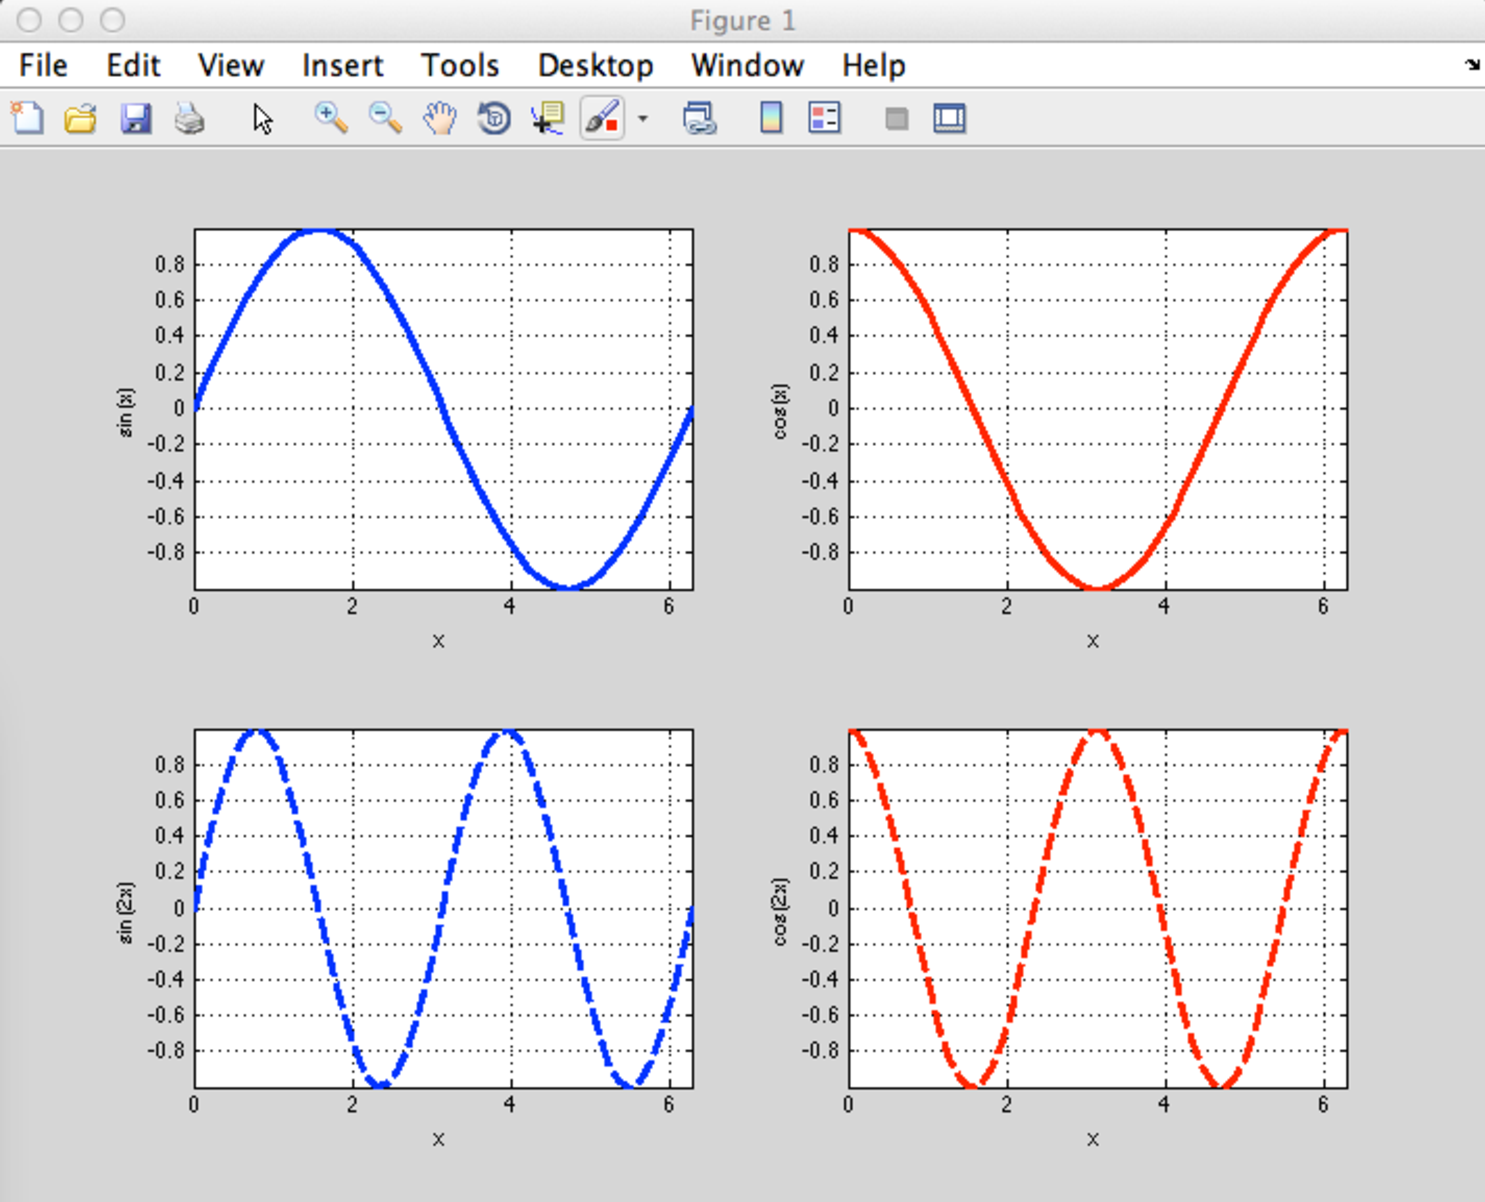
\includegraphics[width=0.9\linewidth]{Graphics/Unit02/subplots}
	\caption{Example of subplots}
	\label{fig:subplots}
\end{figure}

\newpage
%%%%%%%%%%%%%%%%%%%%%%%%%%%%%%%%%%%%%%%%%%%%%%
% Exercise 3: Simple 2D plotting
%%%%%%%%%%%%%%%%%%%%%%%%%%%%%%%%%%%%%%%%%%%%%%
\addtolength{\parindent}{-4mm}
\fcolorbox{myborderblue}{myblue}{%
\begin{minipage}{\linewidth}
\begin{minipage}{6mm}

\includegraphics[scale=0.035]{Graphics/General/exercise_icon}
\end{minipage}
\exercise{\textit{Exercise 3: Simple \twod plotting}} \\
Please save all the plots you produce using the \textit{File \textrightarrow Save} option in the Figure Window. This should save a file with the \mlab default Figure format which uses a \textit{.fig} file extension.
\begin{enumerate}
\item Plot the following functions (you will need to decide on appropriate ranges for $x$):
	\begin{itemize}
	\item $y=\frac{1}{x}$, with a blue dashed line.
	\item $y=\sin(x)\cos(x)$, with a red dotted line.
	\item $y=2x^2-3x+1$, with red cross markers. 
	\end{itemize}
	Turn the \mcode{grid on} in all your plots, and remember to label axes and use a title.
\item Given the following function: \\
\begin{equation*}
s=a \cos(\phi) + \sqrt{b^2 - (a \sin(\phi) - c)^2}
\end{equation*}
Plot $s$ as a function of angle $\phi$ when $a=1$, $b=1.5$, $c=0.3$, and $0 \leq \phi \leq 360^\circ$.
\item Plot the following parametric functions (you will need to use the \mcode{axis equal} command after your \mcode{plot} command to force \mlab to make the x-axis and y-axis the same length):
	\begin{enumerate}
	\item A circle of radius 5 (revisit Ex2 Q7)
	\item \textit{Leminscate} $(-\pi/4 \leq \phi \leq \pi/4)$
		\begin{align*}
		x &= \cos(\phi)\sqrt{2cos(2\phi)} \\
		y &= \sin(\phi)\sqrt{2cos(2\phi)}
		\end{align*}
	\item \textit{Logarithmic Spiral} $(0 \leq \phi \leq 6\pi; k=0.1)$
		\begin{align*}
		x &= e^{k\phi}\cos(\phi) \\
		y &= e^{k\phi}\sin(\phi)
		\end{align*}
	\end{enumerate}
\end{enumerate}
%%%%%%%%%%%%%%%%%%%%%%%%%%%%%%%%%%%%%%%%%%%%%%
% Screencast: Exercise 3 Solutions
%%%%%%%%%%%%%%%%%%%%%%%%%%%%%%%%%%%%%%%%%%%%%%
\begin{minipage}{6mm}

\includegraphics[scale=0.03]{Graphics/General/screencast_icon}
\end{minipage}
\href{http://www.eng.ed.ac.uk/teaching/courses/matlab/unit02/Ex3-Solutions.shtml}{\screencast{Exercise 3 Solutions}}\\
(http://www.eng.ed.ac.uk/teaching/courses/matlab/unit02/Ex3-Solutions.shtml)
\end{minipage}%
}\\
\addtolength{\parindent}{4mm}

\section{Curve-fitting}
\mlab provides a number of powerful options for fitting curves and adding trend-lines to data. The Basic Fitting Graphical User Interface (GUI) can be selected from Figure Windows by selecting \textit{Basic fitting} from the \textit{Tools} menu, and offers common curve-fitting options for \twod plots. More advanced functionality, including \threed fits, can be accessed from the Curve Fitting Toolbox using tools such as \mcode{cftool} (for curve fitting) and \mcode{sftool} (for surface fitting)\footnote{Only basic curve-fitting will be covered in this course.}. \\

%%%%%%%%%%%%%%%%%%%%%%%%%%%%%%%%%%%%%%%%%%%%%%
% Screencast: Basic Curve-fitting
%%%%%%%%%%%%%%%%%%%%%%%%%%%%%%%%%%%%%%%%%%%%%%
\addtolength{\parindent}{-4mm}
\fcolorbox{myborderblue}{myblue}{%
\begin{minipage}{\linewidth}
\begin{minipage}{6mm}

\includegraphics[scale=0.03]{Graphics/General/screencast_icon}
\end{minipage}
\href{http://www.eng.ed.ac.uk/teaching/courses/matlab/unit02/basic-curve-fitting.shtml}{\screencast{Basic Curve-fitting}}\\
(http://www.eng.ed.ac.uk/teaching/courses/matlab/unit02/basic-curve-fitting.shtml)
\end{minipage}%
}\\
\addtolength{\parindent}{4mm}

An alternative to the Basic Fitting GUI are the functions \mcode{polyfit} and \mcode{polyval} which can be used to do basic curve-fitting programmatically. Listing~\ref{lst:polyfit} demonstrates how \mcode{polyfit} can be used to fit a polynomial to a data-set.
\begin{lstlisting}[caption={Syntax of \mcode{polyfit} command},label=lst:polyfit]
coeff = polyfit(xdata,ydata,n);
\end{lstlisting}

\subsubsection{Comments:}
\begin{itemize}
\item \mcode{coeff} is a vector containing the coefficients for the polynomial of best fit, \mcode{xdata} and \mcode{ydata} are vectors containing the independent and dependent variables, and \mcode{n} denotes the degree of the polynomial to be fitted.
\end{itemize}
After using \mcode{polyfit} you can use the \mcode{polyval} function to evaluate the polynomial of best fit, given by the set of coefficients \mcode{coeff}, at specific values of your data. This creates a vector of points of the fitted data, \mcode{y_fit}. Listing~\ref{lst:curve_fitting} and Figure~\ref{fig:curve_fitting} demonstrate the use of both the \mcode{polyfit} and \mcode{polyval} functions. The data used for fitting can be downloaded (\href{http://www.eng.ed.ac.uk/teaching/courses/matlab/data/linear_fit_data.mat}{linear\_fit\_data.mat}) and upon double-clicking the \textit{.mat} file, the data will be loaded into \mlab and assigned to the variables \mcode{x} and \mcode{y}. This data is best fitted using a linear or straight-line fit.
\begin{lstlisting}[caption={Using \mcode{polyfit} and \mcode{polyval} for curve-fitting},label=lst:curve_fitting]
>> coeff = polyfit(x,y,1);
>> y_fit = polyval(coeff,x);
>> plot(x,y,'r+',x,y_fit), grid on, xlabel('x-data'), ...
ylabel('y-data'), title('Basic curve-fitting'), ...
legend('Original data','Line of best fit','Location','SouthEast')
\end{lstlisting}

\subsubsection{Comments:}
\begin{itemize}
\item \mcode{'r+'} plots the \mcode{x} and \mcode{y} data using red crosses.
\item You can insert a legend from the Command Window using the \mcode{legend} command, and specifying the text in the legend using strings.
\end{itemize}
\begin{figure}
	\myfloatalign
	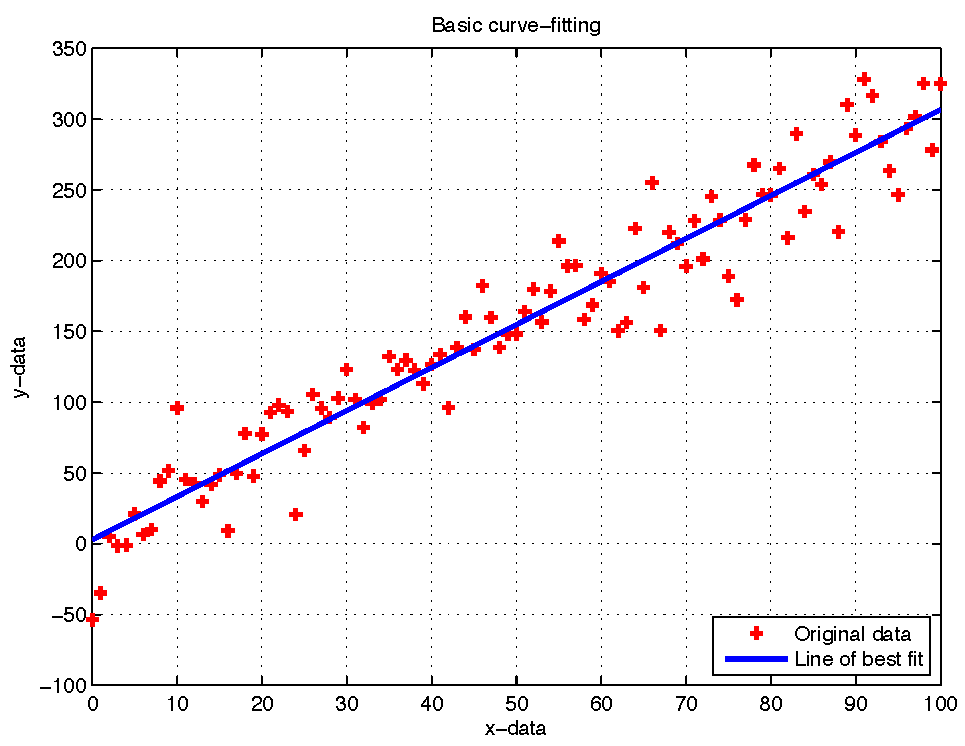
\includegraphics[width=\linewidth]{Graphics/Unit02/curve_fitting}
	\caption{Using \mcode{polyfit} and \mcode{polyval} for curve-fitting}
	\label{fig:curve_fitting}
\end{figure}

\section{\threed plotting using plot3 and surf}
\mlab is hugely powerful and versatile at visualising data in \threed. There are a number of built-in functions for producing different types of  \threed plots \eg\ points, lines, surfaces and volumes.

The \twod \mcode{plot} function becomes \mcode{plot3(x,y,z)} for plotting points and lines in \threed\ space. Listing~\ref{lst:3D-helix} and Figure~\ref{fig:3D-helix} demonstrate using \mcode{plot3} to plot the points on a helix in \threed space.
\begin{lstlisting}[caption={Using \mcode{plot3} to plot points on a helix},label=lst:3D-helix]
>> t = 0:pi/50:10*pi;
>> plot3(sin(t),cos(t),t,'r.'), grid on, ...
xlabel('x'), ylabel('y'), zlabel('z'), title('3D helix')
\end{lstlisting}
\begin{figure}
	\myfloatalign
	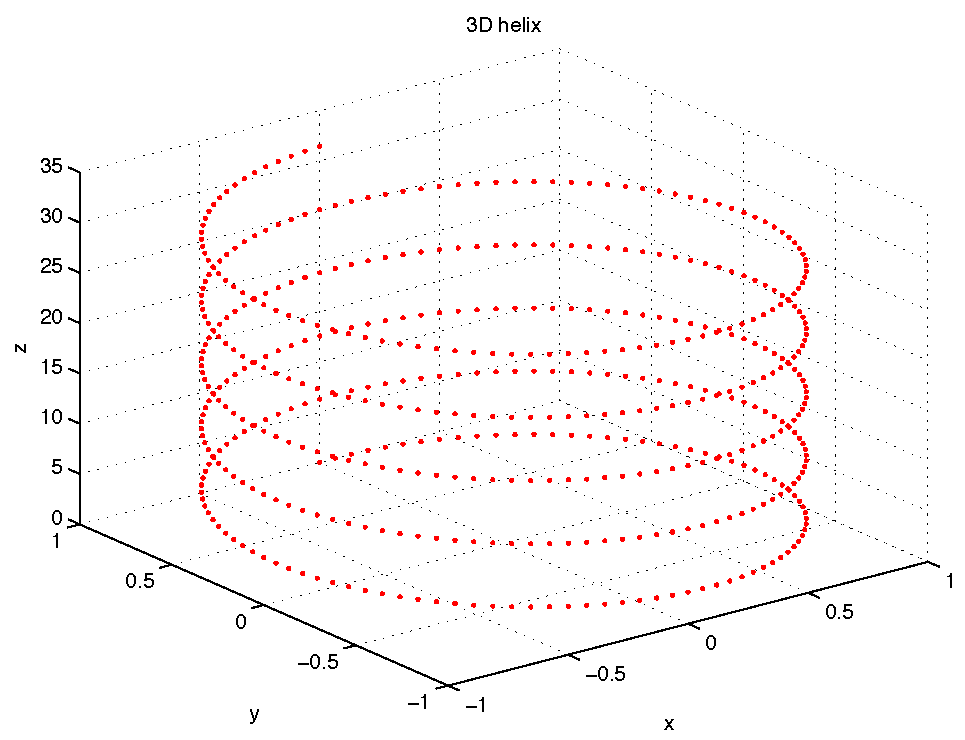
\includegraphics[width=\linewidth]{Graphics/Unit02/3D-helix}
	\caption{Using \mcode{plot3} to plot points on a helix}
	\label{fig:3D-helix}
\end{figure}

For plotting surfaces and contours two commonly used functions are \mcode{surf(x,y,z)} and \mcode{mesh(x,y,z)} where \mcode{x}, \mcode{y}, and \mcode{z} are coordinates of points on a surface. Before you use either of these functions you must use the \mcode{meshgrid} function to define a grid of points which the surface will be plotted onto. Listing~\ref{lst:meshgrid} demonstrates the typical use of \mcode{meshgrid}. In this example, assume $z=f(x,y)$ where $x$ is a vector of values $(1,2,3,4)$ and $y$ is a vector of values $(5,6,7)$. \mcode{meshgrid} takes the vectors $x$ and $y$ and returns two matrices, in this case called $xx$ and $yy$, which contain the coordinates of the grid that the surface $z$ will be plotted onto. Figure~\ref{fig:meshgrid} shows the coordinates of the points in the matrices returned by the \mcode{meshgrid} function.
\begin{figure}
	\myfloatalign
	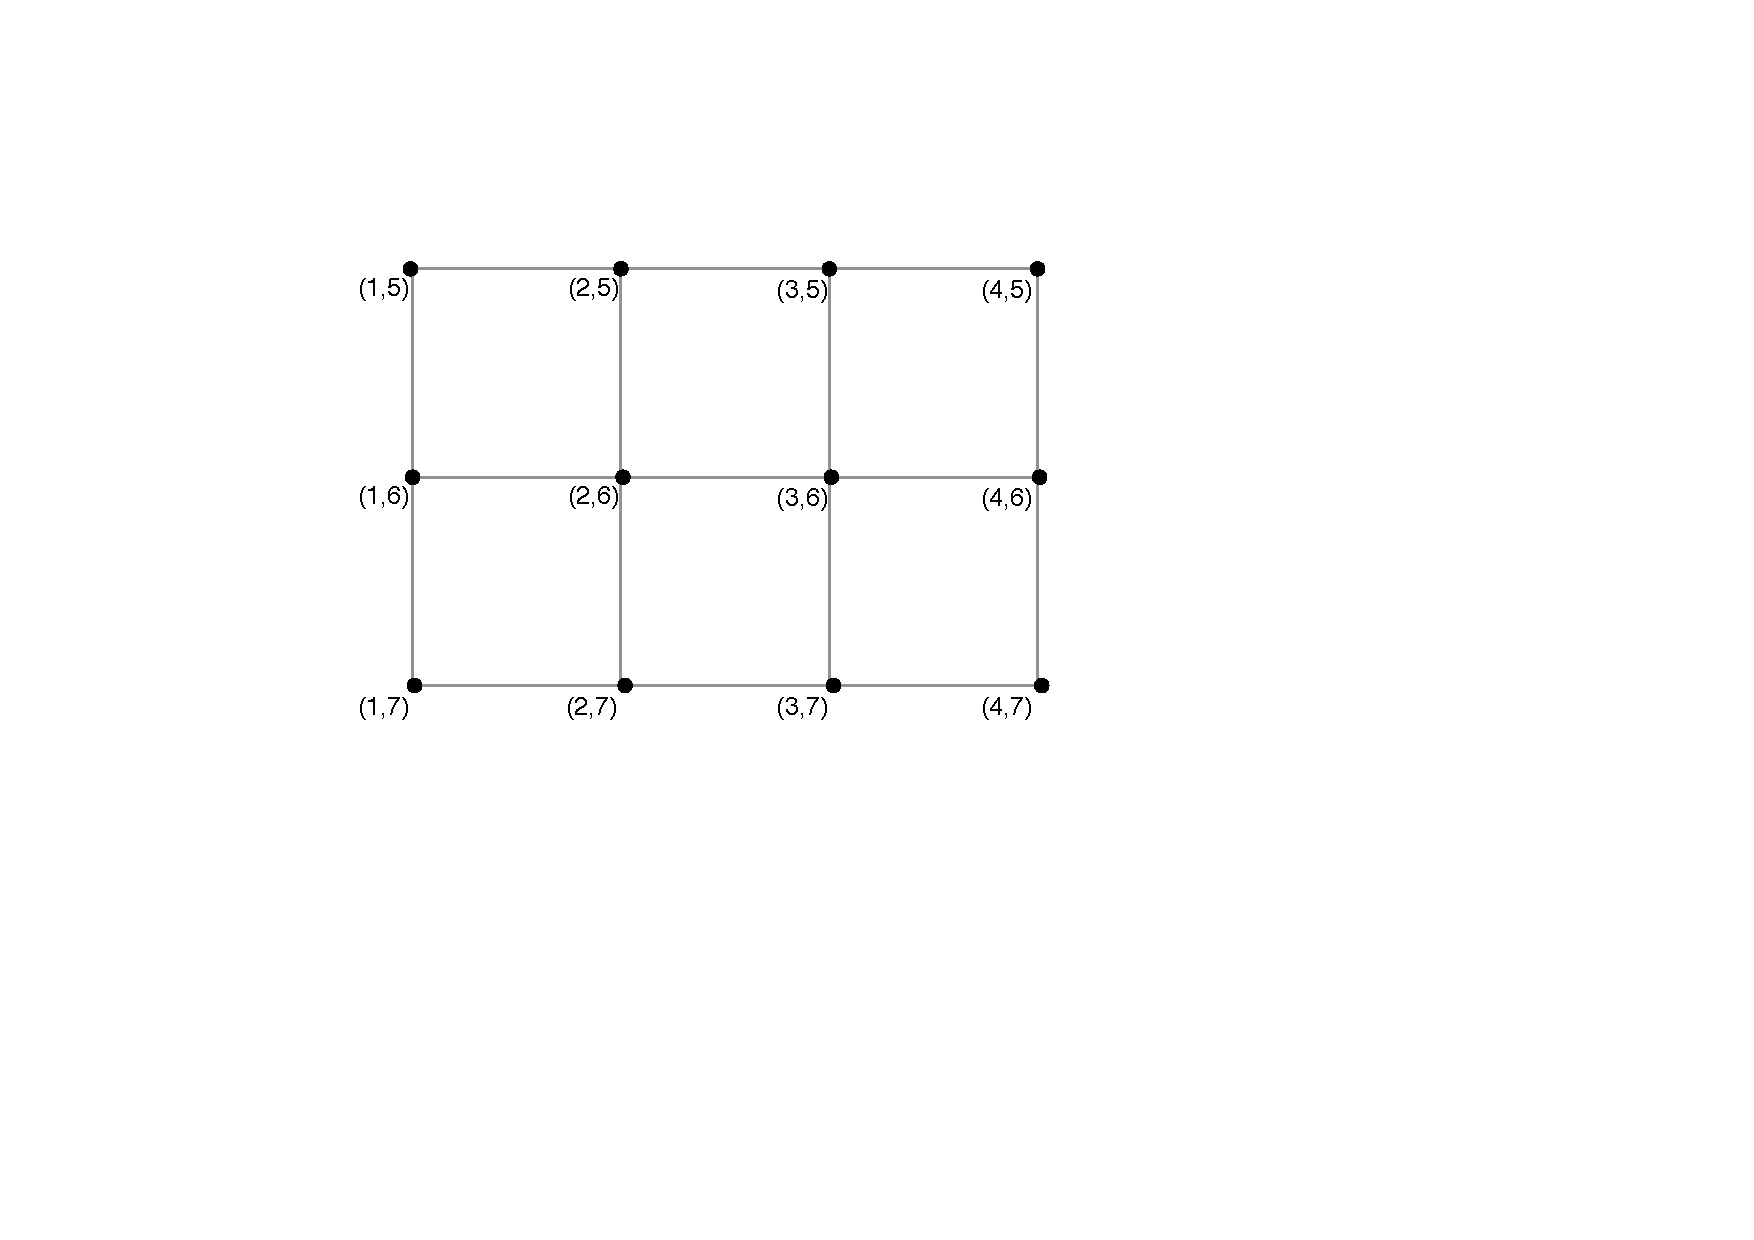
\includegraphics[width=0.70\linewidth]{Graphics/Unit02/meshgrid}
	\caption{Operation of \mcode{meshgrid} function}
	\label{fig:meshgrid}
\end{figure}

\begin{lstlisting}[caption={Using \mcode{meshgrid}},label=lst:meshgrid]
>> x = [1 2 3 4];
>> y = [5 6 7];
>> [xx, yy] = meshgrid(x,y)
xx =
     1     2     3     4
     1     2     3     4
     1     2     3     4
yy =
     5     5     5     5
     6     6     6     6
     7     7     7     7
\end{lstlisting}

\subsubsection{Comments:}
\begin{itemize}
\item \mcode{xx} is an array consisting of rows of the vector \mcode{x}.
\item \mcode{yy} is an array consisting of columns of vector \mcode{y}.
\item \mcode{xx} and \mcode{yy} are then used in the calculation of \mcode{z}, and the plotting of the surface. 
\end{itemize}
Listing~\ref{lst:surf} and Figures~\ref{fig:surf}--\ref{fig:mesh} demonstrate using \mcode{meshgrid} in combination with the surface plotting functions \mcode{surf} (creates a colour-filled surface) and \mcode{mesh} (creates a colored mesh) to plot the function:
\begin{equation*}
z=c \cdot \sin\left( 2\pi a \sqrt{x^2+y^2} \right),
\end{equation*}
where $a=3$, $c=0.5$, $-1\leq x \leq 1$, and $-1\leq y \leq 1$.
\begin{lstlisting}[caption={Plotting a surface},label=lst:surf]
>> x = linspace(-1,1,50);
>> y = x;
>> a = 3;
>> c = 0.5;
>> [xx, yy] = meshgrid(x,y);
>> z = c*sin(2*pi*a*sqrt(xx.^2+yy.^2));
>> surf(xx,yy,z), colorbar, xlabel('x'), ylabel('y'), zlabel('z'), ...
>> title('f(x,y)=csin(2\pia\surd(x^2+y^2))')
>> figure;
>> mesh(xx,yy,z), colorbar, xlabel('x'), ylabel('y'), zlabel('z'), ...
>> title('f(x,y)=csin(2\pia\surd(x^2+y^2))')
\end{lstlisting}
\begin{figure}[h!]
	\myfloatalign
	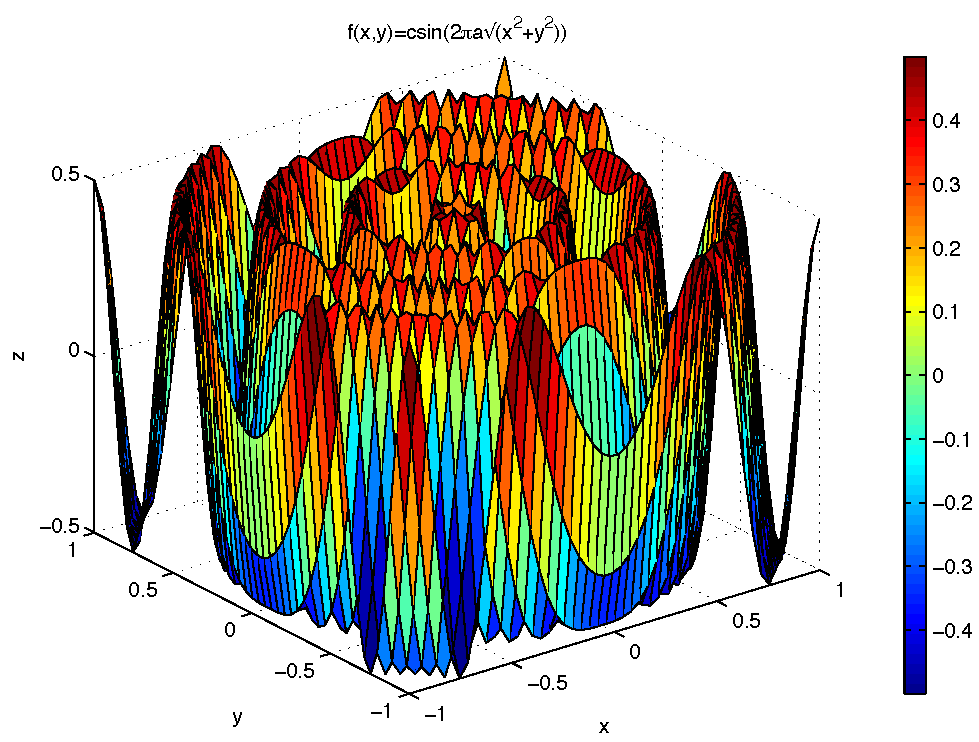
\includegraphics[width=\linewidth]{Graphics/Unit02/surf}
	\caption{Surface plot (using \mcode{surf}) of the function $z=c \cdot \sin( 2\pi a \sqrt{x^2+y^2})$}
	\label{fig:surf}
\end{figure}
\begin{figure}[h!]
	\myfloatalign
	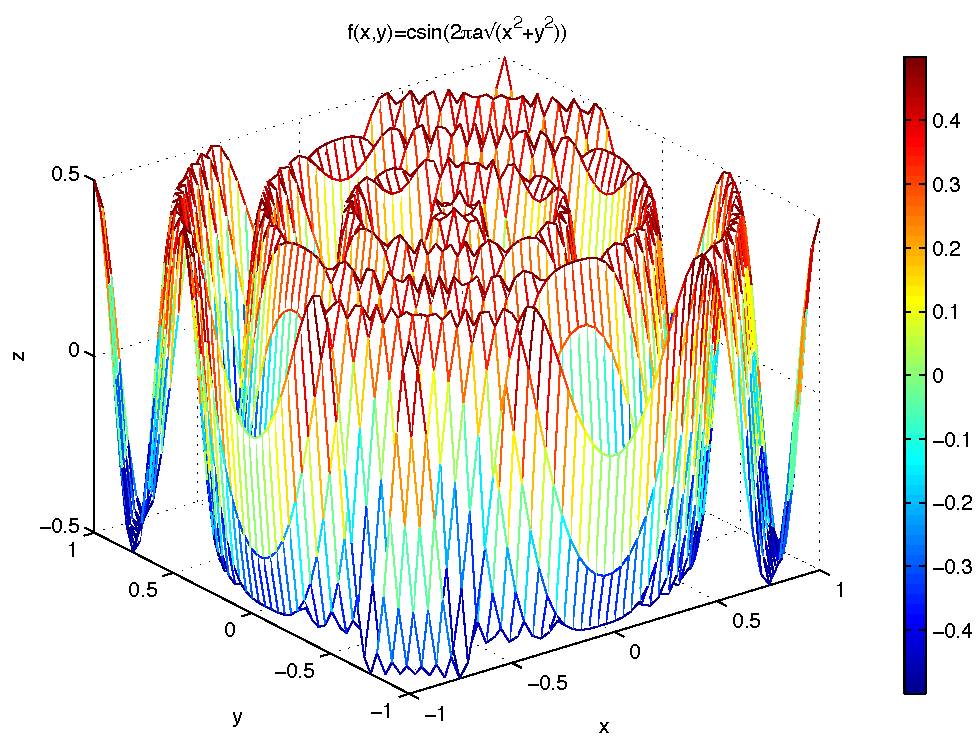
\includegraphics[width=\linewidth]{Graphics/Unit02/mesh}
	\caption{Surface plot (using \mcode{mesh}) of the function $z=c \cdot \sin( 2\pi a \sqrt{x^2+y^2})$}
	\label{fig:mesh}
\end{figure}

%%%%%%%%%%%%%%%%%%%%%%%%%%%%%%%%%%%%%%%%%%%%%%
% Exercise 4: 3D plotting
%%%%%%%%%%%%%%%%%%%%%%%%%%%%%%%%%%%%%%%%%%%%%%
\addtolength{\parindent}{-4mm}
\fcolorbox{myborderblue}{myblue}{%
\begin{minipage}{\linewidth}
\begin{minipage}{6mm}

\includegraphics[scale=0.035]{Graphics/General/exercise_icon}
\end{minipage}
\exercise{\textit{Exercise 4: \threed plotting}}
\begin{enumerate}
\item Plot the following \threed curves using the \mcode{plot3} function:
	\begin{enumerate}
	\item \textit{Spherical helix}
		\begin{align*}
		x&= \sin\left(\frac{t}{2c}\right)\cos(t) \\
		y&= \sin\left(\frac{t}{2c}\right)\sin(t) \\
		z&= \cos\left(\frac{t}{2c}\right)
		\end{align*}
		where $c=5$ and $0 \leq t \leq 10\pi$.
	\item \textit{Sine wave on a sphere}
		\begin{align*}
		x&=\cos(t)\sqrt{b^2-c^2cos^2(at)} \\
		y&=\sin(t)\sqrt{b^2-c^2cos^2(at)} \\
		z&=c*\cos(at)
		\end{align*}
		where $a=10$, $b=1$, $c=0.3$, and $0 \leq t \leq 2\pi$.
	\end{enumerate}

\item Plot the following surfaces using the \mcode{surf} function:
	\begin{enumerate}
	\item \textit{Sine surface}
		\begin{align*}
		x&= \sin(u) \\
		y&= \sin(\nu) \\
		z&= \sin(u+\nu)
		\end{align*}
		where $0 \leq u \leq 2\pi$, and $0 \leq \nu \leq 2\pi$.
	\item \textit{Spring}
		\begin{align*}
		x&= \left[1-r_1 \cos(\nu)\right]\cos(u) \\
		y&= \left[1-r_1 \cos(\nu)\right]\sin(u) \\
		z&= r_2 \left[\sin(\nu)+\frac{tu}{\pi}\right]
		\end{align*}
		where $r_1=r_2=0.5$, $t=1.5$, $0 \leq u \leq 10\pi$, and $0 \leq \nu \leq 10\pi$.
	\item \textit{Elliptic torus}
		\begin{align*}
		x&= \left[c+\cos(\nu)\right]\cos(u) \\
		y&= \left[c+\cos(\nu)\right]\sin(u) \\
		z&= \sin(\nu)\cos(\nu)
		\end{align*}
		where $c=0.5$, $-\pi \leq u \leq \pi$, and $0 \leq \nu \leq \pi$. 
	\end{enumerate}
\end{enumerate}

\end{minipage}%
}\\
\addtolength{\parindent}{4mm}

%%%%%%%%%%%%%%%%%%%%%%%%%%%%%%%%%%%%%%%%%%%%%%
% Exercise 4: 3D plotting (continued)
%%%%%%%%%%%%%%%%%%%%%%%%%%%%%%%%%%%%%%%%%%%%%%
\addtolength{\parindent}{-4mm}
\fcolorbox{myborderblue}{myblue}{%
\begin{minipage}{\linewidth}
\begin{minipage}{6mm}

\includegraphics[scale=0.035]{Graphics/General/exercise_icon}
\end{minipage}
\textit{Exercise 4: \threed plotting (continued)}
\begin{itemize}
	\item Use the \mcode{shading interp} command after \mcode{surf} to change the shading type.
	\item Add a \mcode{colorbar} to the plots.
\end{itemize}	

%%%%%%%%%%%%%%%%%%%%%%%%%%%%%%%%%%%%%%%%%%%%%%
% Screencast: Exercise 4 Solutions
%%%%%%%%%%%%%%%%%%%%%%%%%%%%%%%%%%%%%%%%%%%%%%
\begin{minipage}{6mm}

\includegraphics[scale=0.03]{Graphics/General/screencast_icon}
\end{minipage}
\href{http://www.eng.ed.ac.uk/teaching/courses/matlab/unit02/Ex4-Solutions.shtml}{\screencast{Exercise 4 Solutions}}\\
(http://www.eng.ed.ac.uk/teaching/courses/matlab/unit02/Ex4-Solutions.shtml)
\end{minipage}%
}\\
\addtolength{\parindent}{4mm}

\vspace{5mm}
%%%%%%%%%%%%%%%%%%%%%%%%%%%%%%%%%%%%%%%%%%%%%%
% Reference to additional exercises
%%%%%%%%%%%%%%%%%%%%%%%%%%%%%%%%%%%%%%%%%%%%%%
\addtolength{\parindent}{-4mm}
\fcolorbox{myborderblue}{myblue}{%
\begin{minipage}{\linewidth}
\begin{minipage}{6mm}

\includegraphics[scale=0.035]{Graphics/General/exercise_icon}
\end{minipage}
\textit{Additional Exercises}\\
You should now attempt questions from Chapter~\ref{sect:plotting}. 
\end{minipage}%
}\\
\addtolength{\parindent}{4mm}